\section{Denoising}

\begin{frame}{XRF Denoising}
    \begin{itemize}
        \item \textbf{The Problem:} XRF spectra are often corrupted by Poisson noise and background artifacts (Compton scattering, Bremsstrahlung).
        \item \textbf{The Impact:} Noise can obscure low-intensity peaks, leading to incorrect elemental identification or inaccurate quantification.
        \item \textbf{The Objective:} "Chemical signal recovery": mapping a noisy raw input spectrum to its clean, noise-free ground-truth counterpart.
    \end{itemize}
\end{frame}

\begin{frame}{Denoising Dataset Generator}
    To train robust models, we developed a specialized \textbf{Parallel Dataset Generator}:
    \begin{itemize}
        \item \textbf{Paired Samples:} Generates 2000 pairs of (Noisy, Clean) spectra.
        \item \textbf{Parameter Randomization:} For every sample, the generator varies:
        \begin{itemize}
            \item Signal counts (peak intensity)
            \item Poisson noise levels
            \item Background levels and scattering intensities
            \item Physical parameters (voltage, angle, target material)
        \end{itemize}
        \item \textbf{Generalization:} Randomizing ranges instead of fixed values forces the model to generalize across diverse signal-to-noise ratios.
    \end{itemize}
\end{frame}

\begin{frame}{Preprocessing Strategy}
    XRF spectra present a unique \textbf{"Peak vs. Baseline"} challenge: peaks can be orders of magnitude larger than the background.
    \vspace{0.3cm}
    \begin{block}{Solution: Logarithmic Compression}
        We selected \textbf{LogMinMaxScaler} as the optimal strategy:
        \begin{itemize}
            \item Compresses the dynamic range of massive peaks.
            \item \textbf{Benefit:} Ensures low-intensity peaks are not "drowned out" and remain visible to the model.
        \end{itemize}
    \end{block}
\end{frame}

\begin{frame}{Detailed Model Architectures (1/2)}
    We evaluated 8 diverse architectures to find the best structural fit for 1D spectral data:
    \vspace{0.2cm}
    \begin{itemize}
        \item \textbf{CNN (1D):} Standard convolutional autoencoder. Uses local kernels to detect and "smooth" peak shapes.
        \item \textbf{UNet1D:} Deep encoder-decoder with skip-connections. Excellent for preserving high-resolution peak positions while suppressing noise.
        \item \textbf{Transformer:} Treats spectral channels as a sequence. Uses self-attention to capture long-range dependencies between $K\alpha$ and $K\beta$ lines.
        \item \textbf{Conformer:} State-of-the-art hybrid. Combines local convolutions (shape detection) with global attention (peak relationships).
    \end{itemize}
\end{frame}

\begin{frame}{Detailed Model Architectures (2/2)}
    \begin{itemize}
        \item \textbf{ResNet1D:} Utilizes residual blocks to allow deeper feature extraction without losing original signal information.
        \item \textbf{LSTM:} Recurrent autoencoder. Processes the spectrum as a sequence of energy steps.
        \item \textbf{MLP:} Fully connected autoencoder. Serves as a non-linear baseline.
        \item \textbf{Linear:} Simple linear projection. Provides the ultimate baseline to quantify the value of deep learning.
    \end{itemize}
\end{frame}

\begin{frame}{Loss Function Strategy: Standard MSE + L1}
    \begin{itemize}
        \item \textbf{MSE:} Ensures global reconstruction of the signal across all 600 channels.
        \item \textbf{L1 Sparsity:} Specifically applied to non-peak regions (where ground truth $\approx$ 0).
        \item \textbf{Result:} Forces the background to be sparse (near-zero) while maintaining high peak fidelity.
    \end{itemize}
    \vspace{0.2cm}
    \begin{block}{Why this decision?}
        Standard MSE alone tends to "hallucinate" noise into the baseline. The L1 penalty suppresses these artifacts without affecting peak reconstruction.
    \end{block}
\end{frame}

\begin{frame}{Training Stability: Standard Preprocessing}
    \begin{figure}
        \centering
        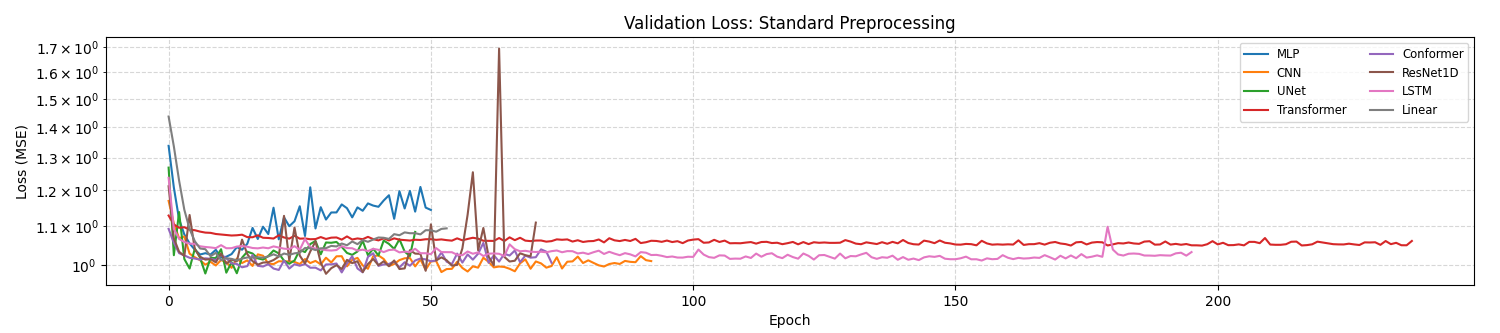
\includegraphics[width=1.0\linewidth]{media/loss_standard.png}
        \caption{Validation loss convergence for all models using Standard scaling.}
    \end{figure}
\end{frame}

\begin{frame}{Training Stability: MinMax Preprocessing}
    \begin{figure}
        \centering
        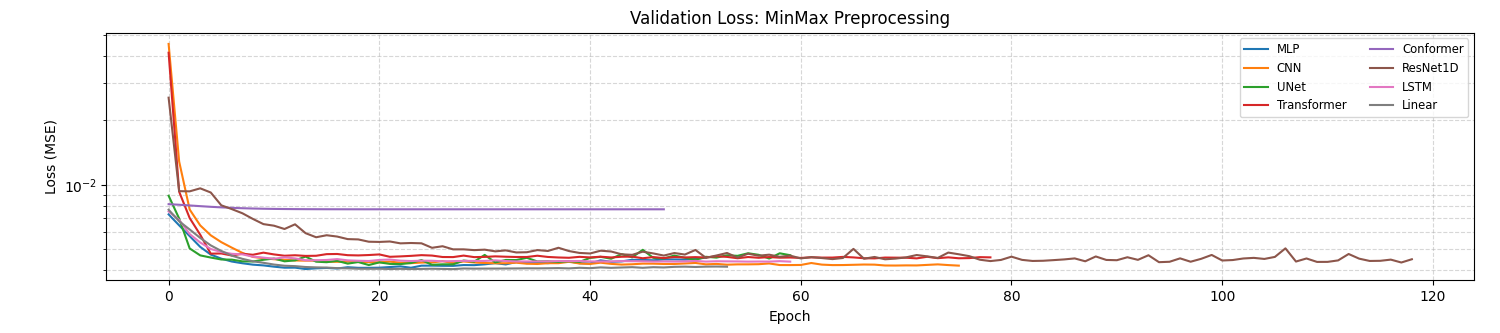
\includegraphics[width=1.0\linewidth]{media/loss_minmax.png}
        \caption{Validation loss convergence for all models using MinMax scaling.}
    \end{figure}
\end{frame}

\begin{frame}{Training Stability: LogMinMax Preprocessing}
    \begin{figure}
        \centering
        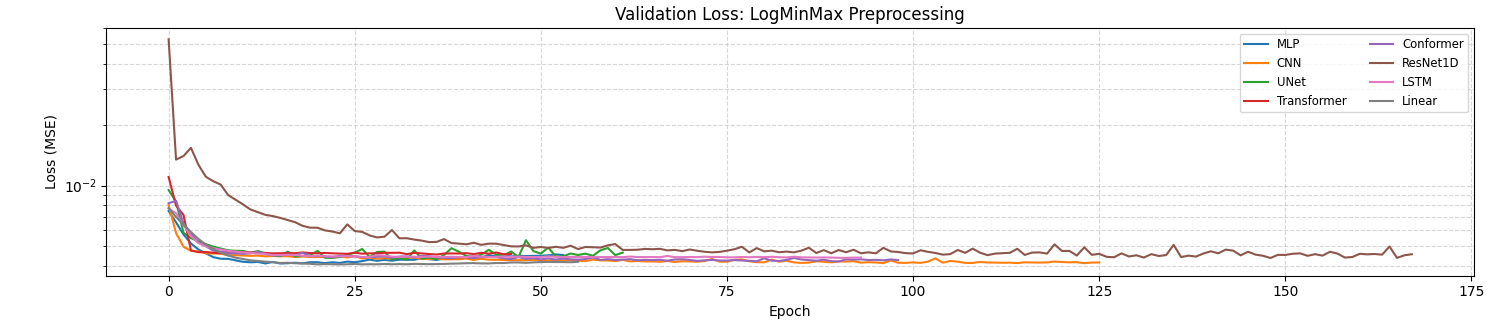
\includegraphics[width=1.0\linewidth]{media/loss_logminmax.png}
        \caption{Validation loss convergence for all models using LogMinMax scaling.}
    \end{figure}
\end{frame}

\begin{frame}{Full Comparative Results: MSE ($\times 10^{-5}$)}
    \centering
    \small
    \begin{table}
        \centering
        \begin{tabular}{lccc}
            \toprule
            \textbf{Architecture} & \textbf{Standard} & \textbf{LogMinMax} & \textbf{MinMax} \\
            \midrule
            CNN & \textbf{3.58} & \textbf{4.38} & 4.71 \\
            Conformer & 3.93 & 4.45 & 11.70 \\
            LSTM & 4.13 & 4.40 & \textbf{4.24} \\
            Linear & 4.19 & 4.77 & 5.12 \\
            Transformer & 4.36 & 4.54 & 4.55 \\
            MLP & 4.37 & 4.92 & 5.21 \\
            UNet1D & 4.88 & 4.63 & 4.46 \\
            ResNet1D & 4.94 & 4.74 & 4.86 \\
            \bottomrule
        \end{tabular}
        \caption{Detailed comparison of MSE across all models and preprocessing strategies.}
    \end{table}
\end{frame}

\begin{frame}{Full Comparative Results: MAE ($\times 10^{-3}$)}
    \centering
    \small
    \begin{table}
        \centering
        \begin{tabular}{lccc}
            \toprule
            \textbf{Architecture} & \textbf{Standard} & \textbf{LogMinMax} & \textbf{MinMax} \\
            \midrule
            UNet1D & \textbf{1.20} & 1.39 & 1.38 \\
            Conformer & 1.22 & 1.30 & 2.40 \\
            CNN & 1.25 & 1.43 & 1.56 \\
            ResNet1D & 1.32 & 1.51 & 1.56 \\
            LSTM & 1.34 & \textbf{1.27} & \textbf{1.29} \\
            Transformer & 1.44 & 1.40 & 1.35 \\
            Linear & 1.66 & 1.64 & 1.71 \\
            MLP & 1.72 & 1.68 & 1.70 \\
            \bottomrule
        \end{tabular}
        \caption{Detailed comparison of MAE across all models and preprocessing strategies.}
    \end{table}
\end{frame}

\begin{frame}{Quantitative Evaluation: MAE Grouped Comparison}
    \begin{figure}
        \centering
        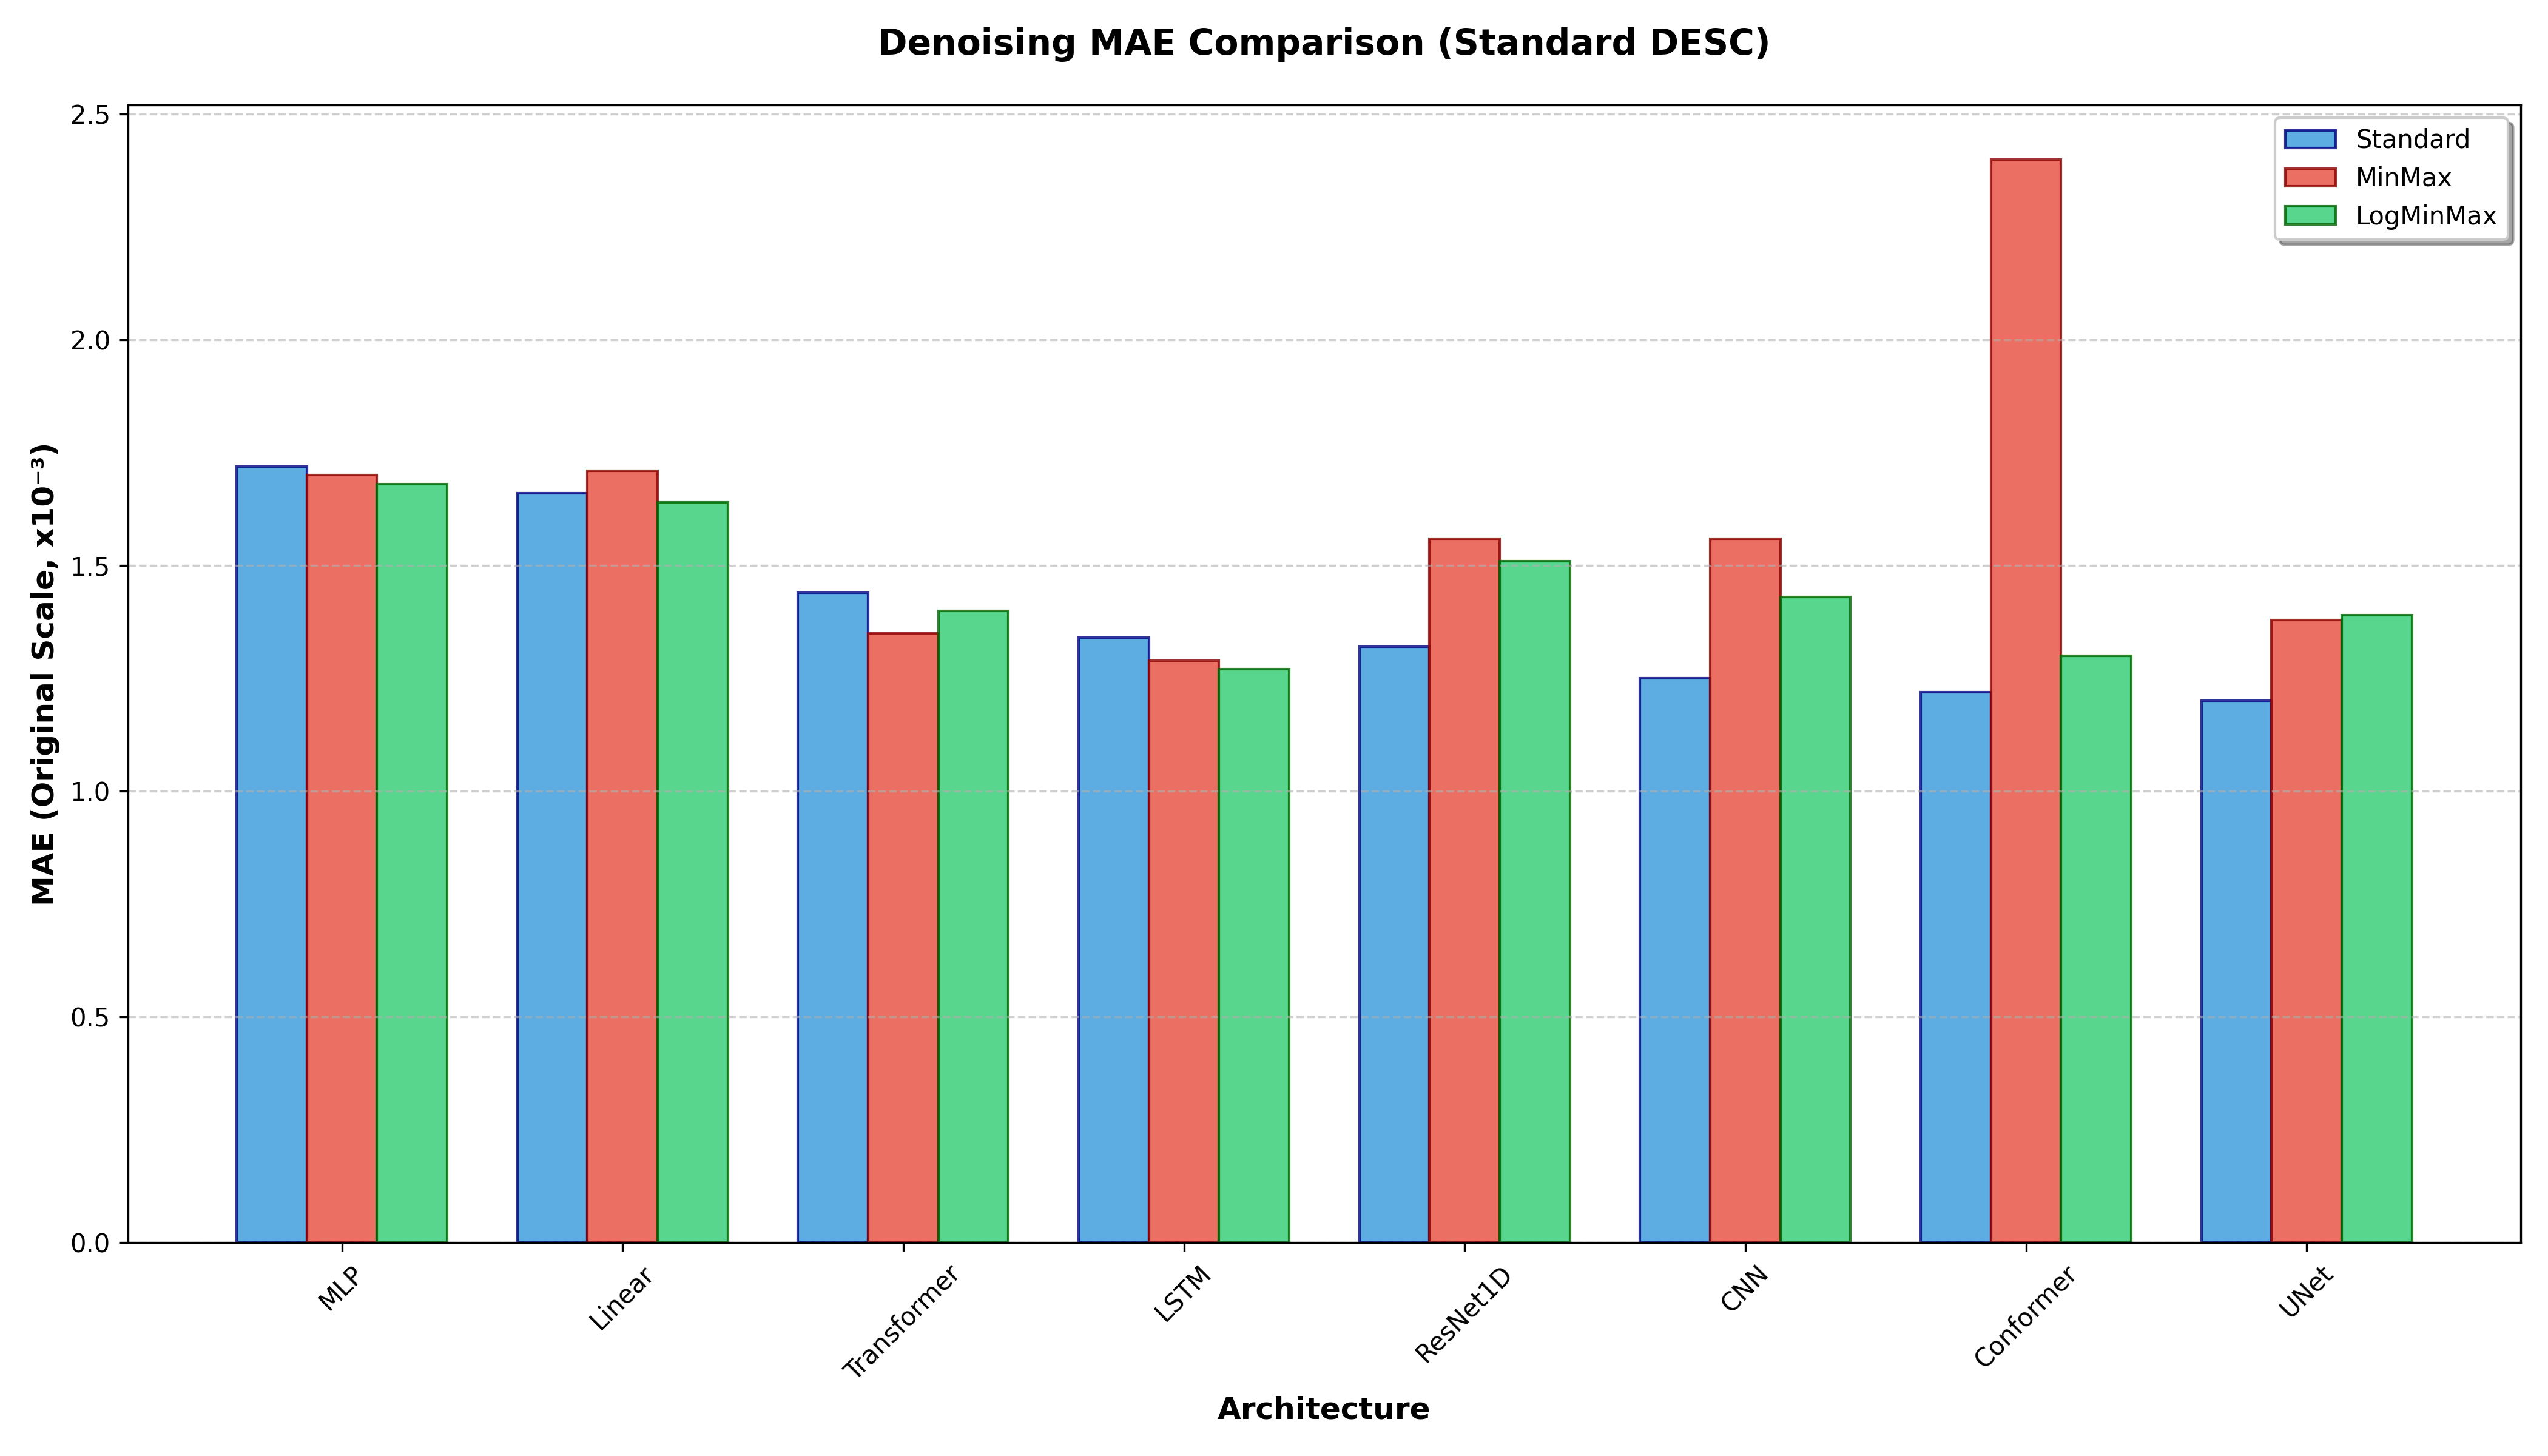
\includegraphics[width=0.9\linewidth]{media/denoising_mae_comparison.png}
        \caption{Impact of preprocessing on architecture performance (MAE Ranking).}
    \end{figure}
\end{frame}

\begin{frame}{Quantitative Evaluation: MSE Grouped Comparison}
    \begin{figure}
        \centering
        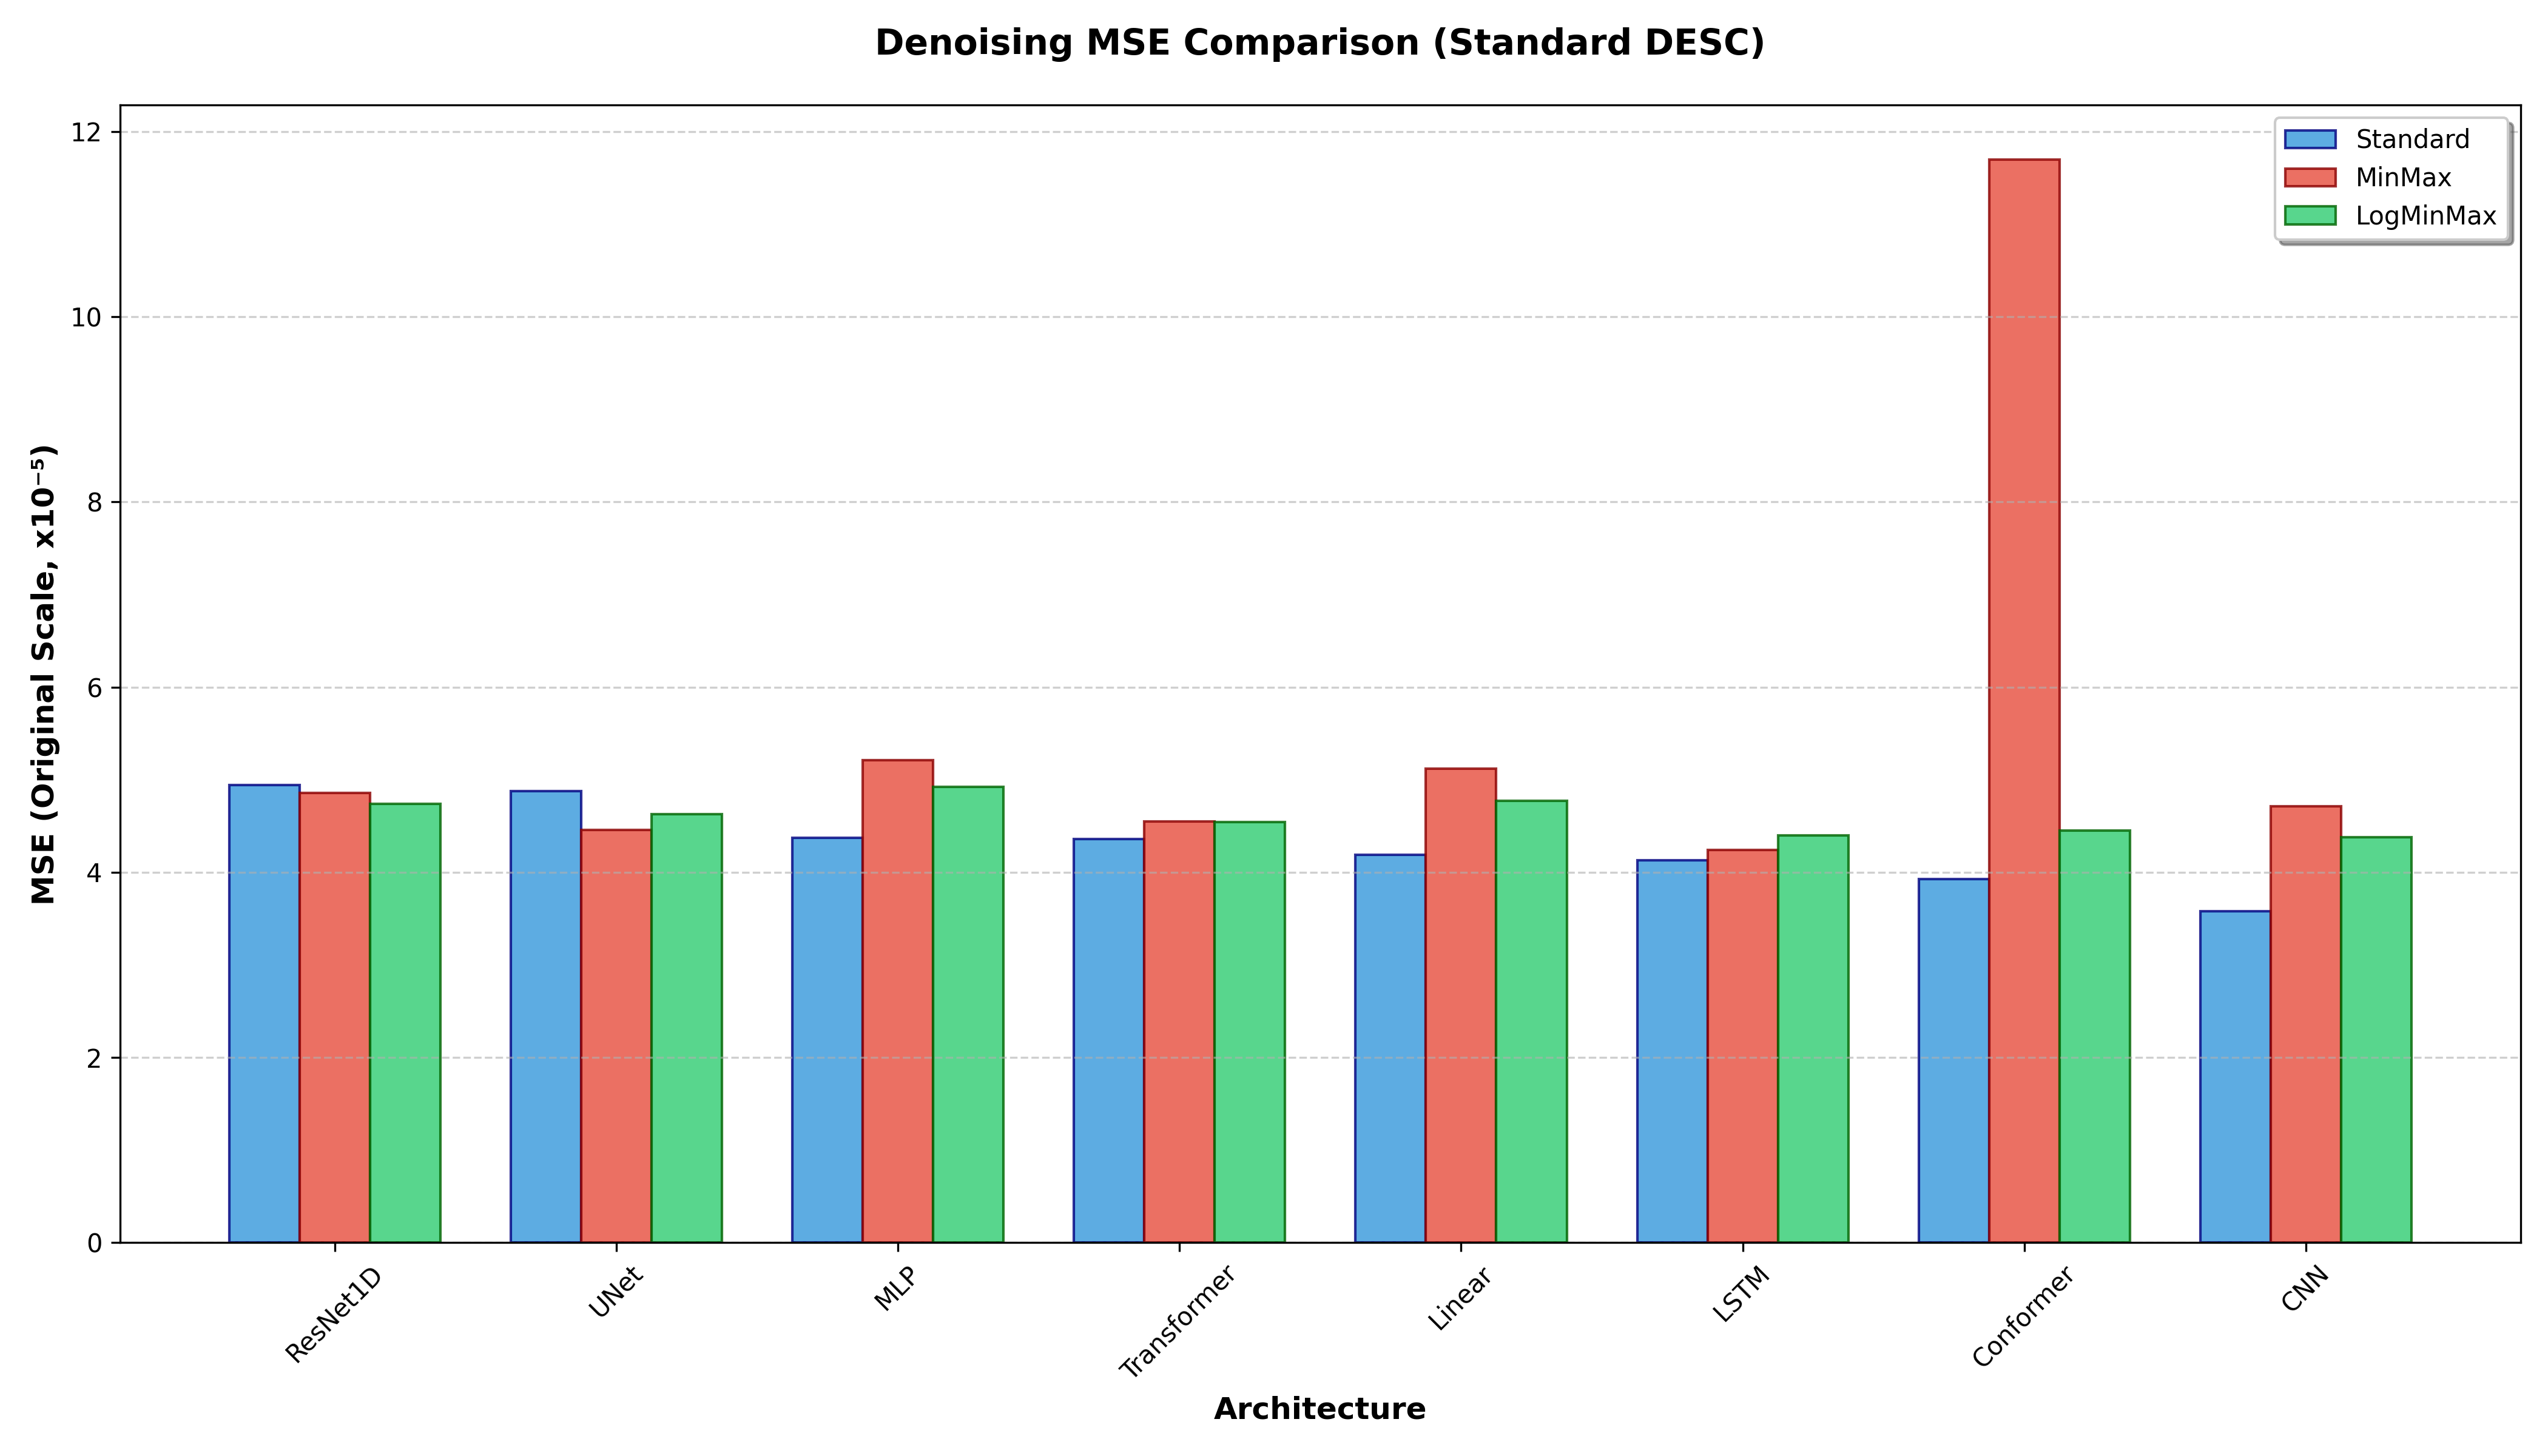
\includegraphics[width=0.9\linewidth]{media/denoising_mse_comparison.png}
        \caption{Impact of preprocessing on architecture performance (MSE Ranking).}
    \end{figure}
\end{frame}

\begin{frame}{Reconstruction Showcase: Best vs Worst Models (MSE)}
    \begin{figure}
        \centering
        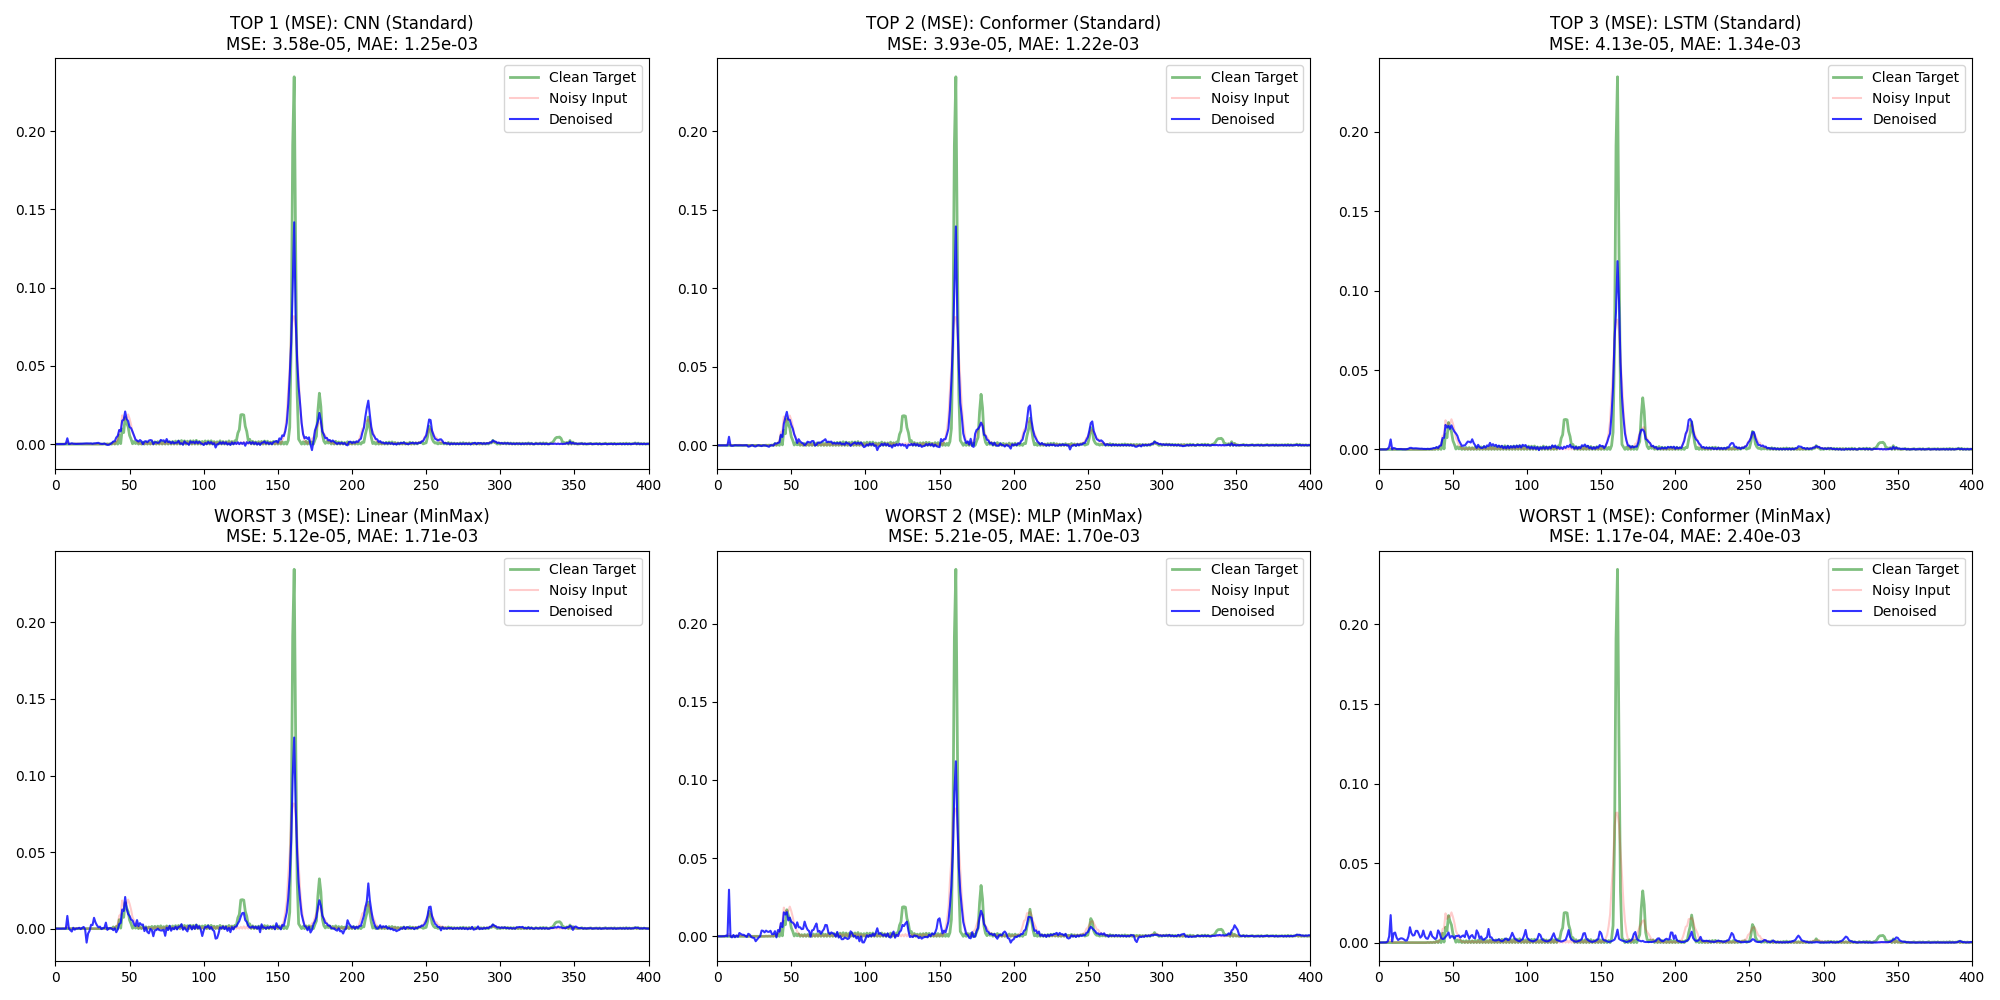
\includegraphics[width=0.95\linewidth]{media/denoising_sample_reconstructions_mse.png}
        \caption{Visual signal recovery for the overall top 3 and worst 3 models (Standard vs MinMax).}
    \end{figure}
\end{frame}

\begin{frame}{The Denoising Champion: CNN + Standard}
    \begin{columns}
        \begin{column}{0.5\textwidth}
            \begin{itemize}
                \item \textbf{Global Fidelity:} Achieved the lowest overall MSE across the entire test set.
                \item \textbf{Local Feature Extraction:} The kernels are exceptionally efficient at modeling and recovering peak shapes.
                \item \textbf{Preprocessing Synergy:} Standard scaling preserves the natural peak-to-background ratio which the CNN leverages for optimal noise separation.
            \end{itemize}
        \end{column}
        \begin{column}{0.5\textwidth}
            \begin{figure}
                \centering
                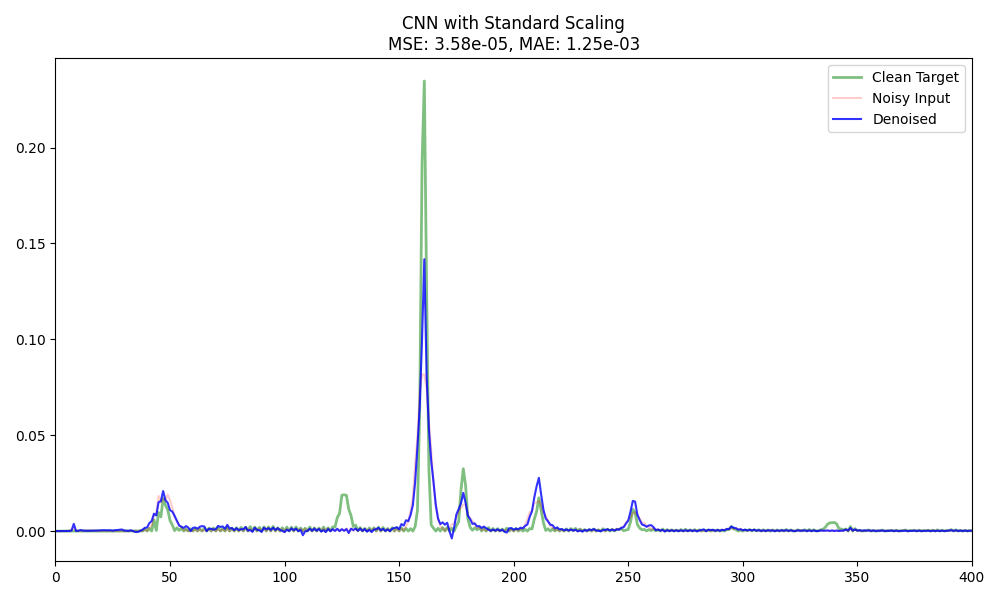
\includegraphics[width=\linewidth]{media/denoising_cnn_sample.png}
                \caption{Superior reconstruction achieved by the CNN Autoencoder.}
            \end{figure}
        \end{column}
    \end{columns}
\end{frame}
